\chapter{Meiose, mistura genética e hereditariedade}\label{ch:b2:meiosis-heredity}

Dois pais de olhos castanhos têm um filho de olhos azuis, e ninguém se
surpreende; dois filhos dos mesmos pais nunca são iguais, e ninguém se
surpreende tampouco. Os dois fatos decorrem de um mesmo processo. Na
formação de cada óvulo e de cada espermatozoide, uma célula com duas
cópias de cada cromossomo transmite exatamente uma, escolhida ao
acaso, depois de deixar as duas cópias trocarem segmentos. Cada
fecundação reúne então dois desses meios conjuntos que nunca se
encontraram. Este capítulo descreve esse processo --- a \omterm{def:b2:meiosis-heredity:meiosis}{meiose} --- e as
regras de herança que dele decorrem: as proporções de Mendel, suas
exceções, a ligação dos genes que compartilham um cromossomo e os
mapas que essa ligação desenha, e a herança peculiar dos \omterm{prop:b2:meiosis-heredity:sexlinked}{cromossomos
sexuais} e das organelas.

\section{A meiose}

\begin{definition}[Meiose]\label{def:b2:meiosis-heredity:meiosis}
\index{meiose}\index{haploide}\index{diploide}
Uma célula \emph{diploide} ($2n$) tem dois cromossomos
\emph{homólogos} de cada tipo, um de cada genitor, iguais quanto ao
conteúdo gênico, mas não necessariamente quanto aos \omterm{def:b2:meiosis-heredity:vocabulary}{alelos}. A
\emph{meiose} é o par de divisões que transforma uma célula diploide
em quatro células \emph{haploides} ($n$), cada uma com um cromossomo de
cada tipo. Ela é precedida por uma única replicação, de modo que cada
cromossomo entra como duas cromátides-irmãs; a primeira divisão separa
os \emph{homólogos} (reducional), a segunda separa as
\emph{cromátides-irmãs} (equacional), como faz a mitose. Nos animais,
a meiose produz gametas; nas plantas e nos fungos, produz esporos
(\cref{ch:b2:plant-life-cycles}); em todo organismo sexuado, é a etapa que reduz à metade o
número de cromossomos para que a fecundação possa dobrá-lo de novo.
\end{definition}

\begin{proposition}[As fases]\label{prop:b2:meiosis-heredity:stages}
\index{prófase I}\index{sinapse}\index{quiasma}\index{crossing-over}
A \emph{\omterm{prop:b2:meiosis-heredity:stages}{prófase I}} é longa, e é nela que ocorre a mistura. Os
cromossomos replicados se condensam; cada um encontra seu homólogo e
pareia com ele gene a gene (\emph{sinapse}), mantido por uma escada
proteica, o \emph{complexo sinaptonêmico}, formando um
\emph{bivalente} de quatro cromátides; cromátides não irmãs se quebram
e se reúnem em pontos correspondentes (\emph{crossing-over}), uma a
várias vezes por bivalente; quando o complexo se desfaz, os homólogos
permanecem unidos apenas nesses pontos de troca, visíveis como
\emph{quiasmas}. \emph{Metáfase I}: os bivalentes se alinham no fuso,
cada par orientado ao acaso --- o homólogo materno voltado para um
polo ou para o outro, independentemente de todos os outros pares.
\emph{Anáfase I}: os homólogos se separam, e as cromátides-irmãs
permanecem juntas; cada polo recebe $n$ cromossomos de duas
cromátides cada. \emph{Telófase I} e, geralmente sem replicação,
\emph{\omterm{def:b2:meiosis-heredity:meiosis}{meiose} II}: os $n$ cromossomos se alinham um a um, as
cromátides-irmãs se separam e resultam quatro núcleos \omterm{def:b2:meiosis-heredity:meiosis}{haploides}. A
\omterm{def:b2:meiosis-heredity:meiosis}{meiose} I dura de horas a décadas (um ovócito humano fica parado em
\omterm{prop:b2:meiosis-heredity:stages}{prófase I} desde antes do nascimento até a ovulação); a \omterm{def:b2:meiosis-heredity:meiosis}{meiose} II dura
uma hora.
\end{proposition}

\begin{omfigure}
\begin{tikzpicture}[every node/.style={font=\scriptsize}]
  % helper: cell outline at (x,y)
  \foreach \x/\lab in {0/{prófase I: pareamento, crossing-over}, 3.2/{metáfase I: bivalentes alinhados}, 6.4/{anáfase I: os homólogos se separam}, 9.6/{meiose II: as cromátides se separam}}
    { \draw[thick] (\x+1.2,0) circle (1.15); \node[below, align=center, text width=2.8cm] at (\x+1.2,-1.2) {\lab}; }
  % prophase I: one bivalent with chiasma
  \draw[very thick, omDef] (0.8,-0.5) -- (0.8,0.5); \draw[very thick, omDef] (1.0,-0.5) -- (1.0,0.5);
  \draw[very thick, omThm] (1.4,-0.5) -- (1.4,0.5); \draw[very thick, omThm] (1.6,-0.5) -- (1.6,0.5);
  \draw[very thick, omDef] (1.0,0.1) -- (1.4,-0.1); \draw[very thick, omThm] (1.4,0.1) -- (1.0,-0.1);
  \fill[white] (0.9,-0.03) rectangle (1.5,0.03);
  \draw[very thick, omDef] (1.0,0.1) -- (1.4,-0.1); \draw[very thick, omThm] (1.4,0.1) -- (1.0,-0.1);
  \node[omExo!60!black] at (1.2,-0.85) {quiasma};
  % metaphase I: two bivalents on the plate, spindle
  \begin{scope}[xshift=3.2cm]
    \draw[gray, dashed] (1.2,-1.0) -- (1.2,1.0);
    \foreach \y in {0.45,-0.45} {
      \draw[very thick, omDef] (0.95,\y-0.25) -- (0.95,\y+0.25); \draw[very thick, omDef] (1.08,\y-0.25) -- (1.08,\y+0.25);
      \draw[very thick, omThm] (1.32,\y-0.25) -- (1.32,\y+0.25); \draw[very thick, omThm] (1.45,\y-0.25) -- (1.45,\y+0.25);
    }
    \draw[gray] (0.15,0) -- (0.95,0.45); \draw[gray] (0.15,0) -- (0.95,-0.45);
    \draw[gray] (2.25,0) -- (1.45,0.45); \draw[gray] (2.25,0) -- (1.45,-0.45);
  \end{scope}
  % anaphase I
  \begin{scope}[xshift=6.4cm]
    \foreach \y in {0.45,-0.45} {
      \draw[very thick, omDef] (0.45,\y-0.25) -- (0.45,\y+0.25); \draw[very thick, omDef] (0.58,\y-0.25) -- (0.58,\y+0.25);
      \draw[very thick, omThm] (1.82,\y-0.25) -- (1.82,\y+0.25); \draw[very thick, omThm] (1.95,\y-0.25) -- (1.95,\y+0.25);
    }
    \draw[->, gray] (1.2,0) -- (0.75,0); \draw[->, gray] (1.2,0) -- (1.65,0);
  \end{scope}
  % meiosis II: four cells
  \begin{scope}[xshift=9.6cm]
    \foreach \p/\c in {(0.75,0.5)/omDef,(1.65,0.5)/omDef,(0.75,-0.5)/omThm,(1.65,-0.5)/omThm} {
      \draw[thick, gray!60] \p circle (0.38);
      \draw[very thick, \c] \p ++(-0.12,-0.2) -- ++(0,0.4);
      \draw[very thick, \c] \p ++(0.12,-0.2) -- ++(0,0.4);
    }
  \end{scope}
\end{tikzpicture}

{\small A \omterm{def:b2:meiosis-heredity:meiosis}{meiose} para dois pares de homólogos (maternos em azul,
paternos em vermelho, cada um com duas cromátides). Os homólogos
pareiam e trocam segmentos na \omterm{prop:b2:meiosis-heredity:stages}{prófase I}, alinham-se como bivalentes na
metáfase I e se separam na anáfase I; a \omterm{def:b2:meiosis-heredity:meiosis}{meiose} II separa as cromátides
em quatro células \omterm{def:b2:meiosis-heredity:meiosis}{haploides}.}
\end{omfigure}

\begin{omfigure}
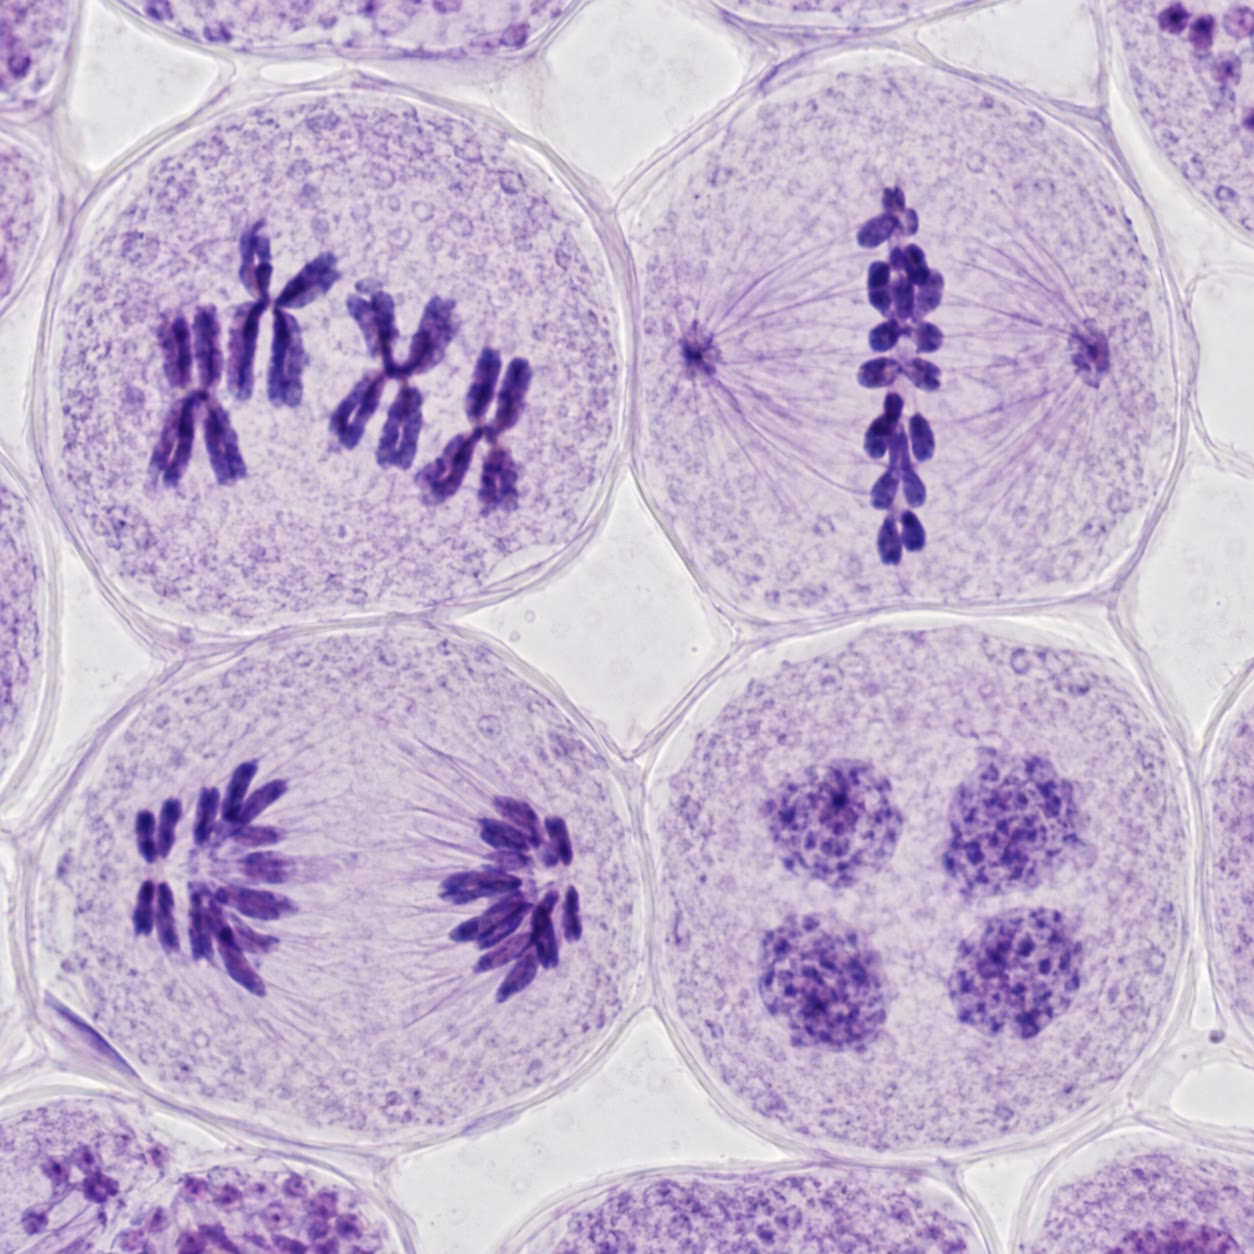
\includegraphics[width=0.5\linewidth]{images/book4/ai/b4-04-lily-meiosis.jpg}

{\small A \omterm{def:b2:meiosis-heredity:meiosis}{meiose} na antera de um lírio: bivalentes no fim da \omterm{prop:b2:meiosis-heredity:stages}{prófase
I}, uma placa de metáfase I, a anáfase I e os quatro núcleos de uma
tétrade.}
\end{omfigure}

\begin{theorem}[Quanta mistura a meiose produz]\label{thm:b2:meiosis-heredity:mixing}
\index{segregação independente}\index{recombinação genética}
Para um organismo com $n$ pares de cromossomos, a orientação aleatória
dos bivalentes na metáfase I produz $2^n$ combinações possíveis de
cromossomos maternos e paternos num gameta ---
$2^{23} \approx 8.4$ milhões num ser humano --- e $2^{2n}$ num zigoto.
O crossing-over multiplica esse número: com cerca de $k$ quiasmas por
bivalente, cada um numa posição variável, o número de gametas
distintos é na prática ilimitado, e dois gametas de uma mesma pessoa
nunca são iguais. A \emph{recombinação} --- novas combinações de
\omterm{def:b2:meiosis-heredity:vocabulary}{alelos} --- decorre de ambos: a \omterm{thm:b2:meiosis-heredity:mixing}{segregação independente} reembaralha
cromossomos inteiros, o crossing-over reembaralha genes dentro de um
cromossomo.
\end{theorem}
\begin{proof}
Cada bivalente se orienta de modo independente, com dois resultados
possíveis, de modo que $n$ bivalentes dão $2^n$ combinações, todas
igualmente prováveis. Cada um dos dois genitores contribui com um
desses gametas, de modo que o zigoto tem $2^n\times
2^n$. Um crossing-over numa posição distinta de um cromossomo de $L$
pares de bases pode produzir da ordem de $L$ cromátides recombinantes
distintas por bivalente, de modo que o número de produtos distintos
cresce como $L^k$ por cromossomo, o que é astronômico para
$L \sim 10^8$.
\end{proof}
\begin{proof}[Evidências]
Creighton e McClintock (1931) usaram um cromossomo 9 de milho que
levava duas marcas citológicas visíveis (um nó numa extremidade, um
segmento translocado na outra) e dois genes entre elas (grão colorido
ou incolor, endosperma ceroso ou amiláceo). Entre os descendentes,
toda planta com um par de \omterm{def:b2:meiosis-heredity:vocabulary}{alelos} recombinado tinha também um par de
marcas citológicas recombinado --- nó sem translocação ou o inverso
---, o que provou que a \omterm{thm:b2:meiosis-heredity:mixing}{recombinação genética} é uma troca física de
segmentos cromossômicos.
\end{proof}

\begin{omfigure}
\begin{tikzpicture}[every node/.style={font=\scriptsize}]
  \foreach \dx/\lab/\ca/\cb/\gam in {0/{orientação 1}/omDef/omThm/{gametas AB e ab}, 6.2/{orientação 2}/omThm/omDef/{gametas Ab e aB}} {
    \begin{scope}[xshift=\dx cm]
      \draw[gray, dashed] (0,-1.1) -- (3.2,-1.1);
      \node[anchor=south] at (1.6,0.6) {\lab};
      % pair 1 (long): A above the plate, a below
      \draw[very thick, omDef] (0.7,-0.95) -- (0.7,-0.25); \node[omDef, anchor=south] at (0.7,-0.2) {A};
      \draw[very thick, omThm] (0.7,-1.25) -- (0.7,-1.95); \node[omThm, anchor=north] at (0.7,-2.0) {a};
      % pair 2 (short): B or b above depending on orientation
      \draw[very thick, \ca] (2.3,-0.85) -- (2.3,-0.35);
      \draw[very thick, \cb] (2.3,-1.35) -- (2.3,-1.85);
      \node[anchor=north] at (1.6,-2.4) {\gam};
    \end{scope}
  }
  \node[omDef, anchor=south] at (2.3,-0.3) {B}; \node[omThm, anchor=north] at (2.3,-1.9) {b};
  \node[omThm, anchor=south] at (8.5,-0.3) {b}; \node[omDef, anchor=north] at (8.5,-1.9) {B};
  \node[anchor=north, align=center] at (4.7,-3.0) {cada orientação igualmente provável:\\gametas AB, ab, Ab, aB em números iguais --- segregação independente};
\end{tikzpicture}

{\small A \omterm{thm:b2:meiosis-heredity:mixing}{segregação independente}. Para dois pares de cromossomos
(A/a num, B/b no outro), as duas orientações possíveis dos bivalentes
na metáfase I são igualmente prováveis, de modo que as quatro
combinações de \omterm{def:b2:meiosis-heredity:vocabulary}{alelos} aparecem em números iguais entre os gametas.}
\end{omfigure}

\section{A análise mendeliana}

\begin{definition}[O vocabulário dos cruzamentos]\label{def:b2:meiosis-heredity:vocabulary}
\index{alelo}\index{genótipo}\index{fenótipo}\index{dominante}\index{recessivo}\index{homozigoto}\index{heterozigoto}
Um \emph{gene} é um trecho de cromossomo; seus \emph{alelos} são suas
variantes de sequência; o \emph{loco} é sua posição. Um indivíduo
\omterm{def:b2:meiosis-heredity:meiosis}{diploide} tem dois alelos em cada loco: seu \emph{genótipo} é
\emph{homozigoto} ($AA$, $aa$) ou \emph{heterozigoto} ($Aa$). O
\emph{fenótipo} é o caráter observável. Um alelo é
\emph{dominante} quando o heterozigoto exibe seu fenótipo, e
\emph{recessivo} quando só se manifesta no homozigoto; a distinção é
uma propriedade do par de alelos e do caráter observado, e não do
alelo isolado --- a maioria dos alelos recessivos são alelos de perda
de função, mascarados porque uma única cópia funcional basta. Uma
\emph{linhagem pura} se reproduz sem variação (é homozigota); um
\emph{cruzamento-teste} cruza um indivíduo de fenótipo dominante com
um homozigoto recessivo, de modo que seus descendentes revelam
diretamente os alelos de seus gametas.
\end{definition}

\begin{theorem}[As proporções de Mendel]\label{thm:b2:meiosis-heredity:mendel}
\index{leis de Mendel}\index{cruzamento mono-híbrido}\index{cruzamento di-híbrido}
Como os dois \omterm{def:b2:meiosis-heredity:vocabulary}{alelos} de um \omterm{def:b2:meiosis-heredity:vocabulary}{heterozigoto} $Aa$ segregam para gametas
diferentes em números iguais (anáfase I), um cruzamento
\emph{mono-híbrido} $Aa \times Aa$ dá os \omterm{def:b2:meiosis-heredity:vocabulary}{genótipos}
$\tfrac14 AA : \tfrac12 Aa :
\tfrac14 aa$ e os \omterm{def:b2:meiosis-heredity:vocabulary}{fenótipos} $3 : 1$ se $A$ for \omterm{def:b2:meiosis-heredity:vocabulary}{dominante}; o
cruzamento-teste $Aa \times aa$ dá $1 : 1$. Como os \omterm{def:b2:meiosis-heredity:vocabulary}{alelos} de genes
situados em cromossomos diferentes segregam de modo independente
(metáfase I), um \emph{di-híbrido} $AaBb$ produz quatro tipos de
gameta em números iguais, e o cruzamento $AaBb \times AaBb$ dá os
\omterm{def:b2:meiosis-heredity:vocabulary}{fenótipos} $9 : 3 : 3 : 1$; o cruzamento-teste
$AaBb \times aabb$ dá $1 : 1 : 1 : 1$. Para $k$ locos \omterm{def:b2:meiosis-heredity:vocabulary}{heterozigotos}
independentes, o número de tipos de gameta é $2^k$ e a proporção
fenotípica é o produto de $k$ proporções $3 : 1$.
\end{theorem}
\begin{proof}
Segregação: os gametas do \omterm{def:b2:meiosis-heredity:vocabulary}{heterozigoto} são $\tfrac12 A$,
$\tfrac12 a$; com fecundação ao acaso, os \omterm{def:b2:meiosis-heredity:vocabulary}{genótipos} dos zigotos são os
produtos $(\tfrac12 A + \tfrac12 a)^2 = \tfrac14 AA + \tfrac12 Aa +
\tfrac14 aa$. Independência: os gametas de $AaBb$ são $(\tfrac12 A
+ \tfrac12 a)(\tfrac12 B + \tfrac12 b)$, quatro tipos a $\tfrac14$;
os \omterm{def:b2:meiosis-heredity:vocabulary}{fenótipos} do di-híbrido multiplicam $(\tfrac34 A\_ + \tfrac14 aa)
(\tfrac34 B\_ + \tfrac14 bb)$, dando $\tfrac{9}{16}, \tfrac{3}{16},
\tfrac{3}{16}, \tfrac{1}{16}$. Cada fator é uma \omterm{thm:b2:meiosis-heredity:mixing}{segregação
independente}, de modo que $k$ locos dão um produto de $k$ fatores.
\end{proof}
\begin{proof}[Evidências]
Mendel (1866) cruzou linhagens puras de ervilha que diferiam num único
caráter --- semente lisa ou rugosa, cotilédone amarelo ou verde, flor
púrpura ou branca, caule alto ou anão, e outros três --- e encontrou
em todos os casos uma primeira geração uniforme e uma segunda geração
que segregava perto de $3 : 1$: 5474 lisas para 1850 rugosas ($2.96 :
1$), 6022 amarelas para 2001 verdes ($3.01 : 1$), 705 púrpuras para 224
brancas ($3.15 : 1$). Nos cruzamentos com dois caracteres, encontrou
$315 : 108 : 101 :
32$ ($9 : 3 : 3 : 1$) e, cultivando a segunda geração, mostrou que a
classe \omterm{def:b2:meiosis-heredity:vocabulary}{dominante} era de dois tipos, um terço pura e dois terços
segregante. Os cromossomos que explicam as proporções foram
descobertos quarenta anos depois.
\end{proof}

\begin{omfigure}
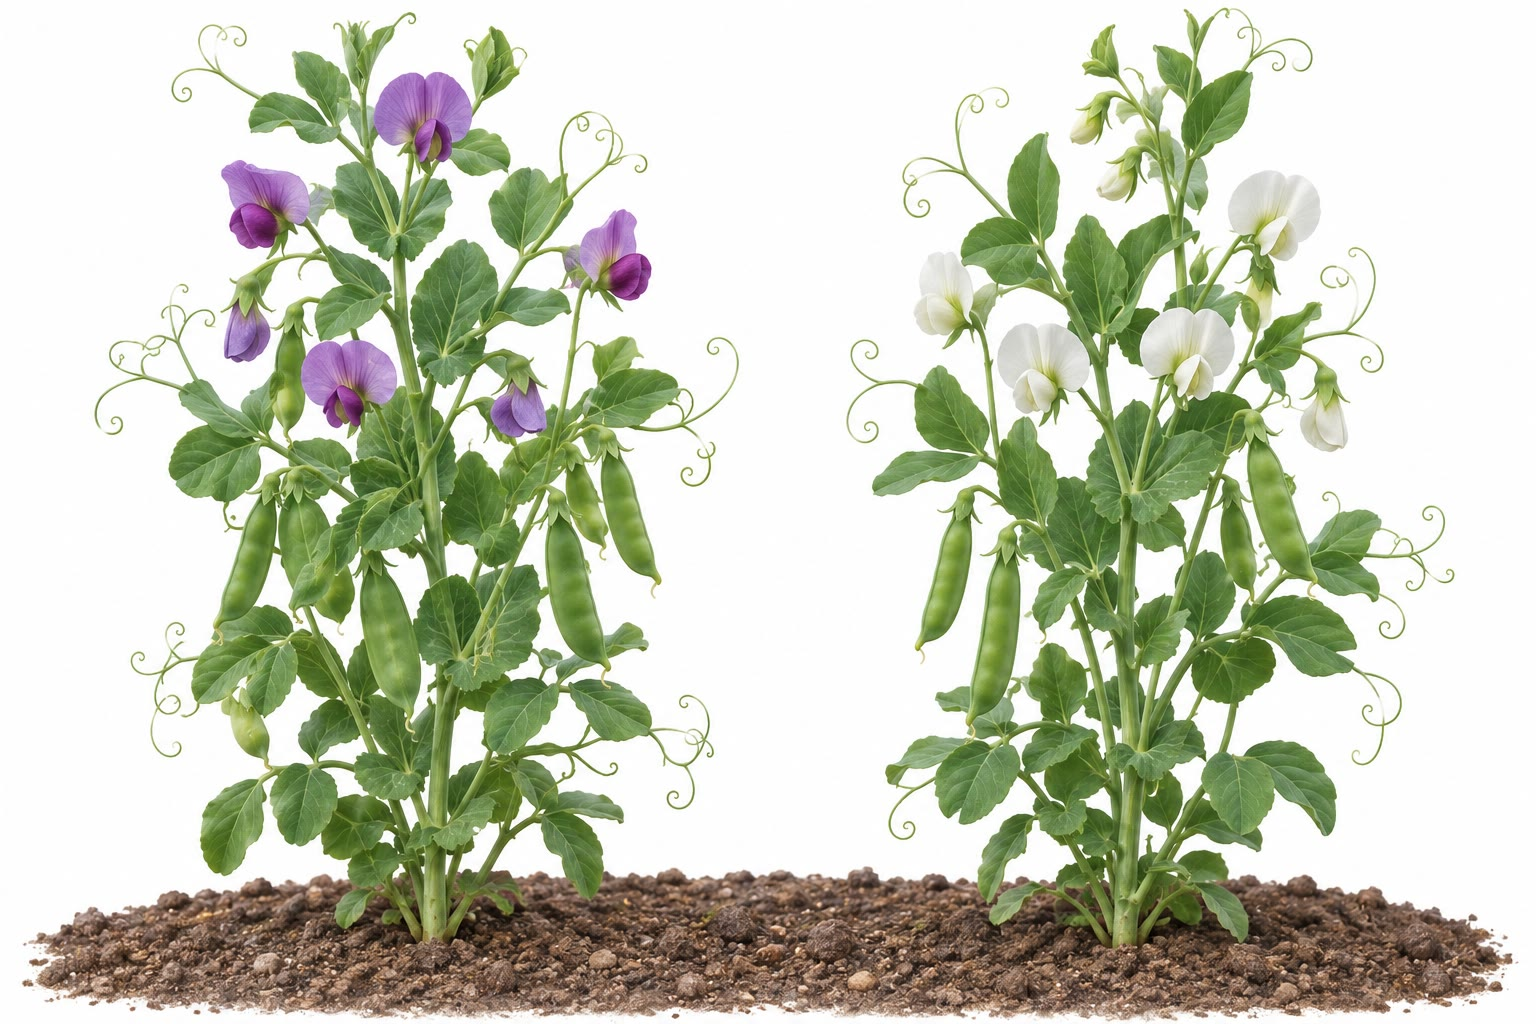
\includegraphics[width=0.58\linewidth]{images/book4/ai/b4-04-pea-flowers.jpg}

{\small Plantas de ervilha de flores púrpuras e de flores brancas: um
dos sete pares de caracteres sobre os quais Mendel fundou a genética.
O híbrido de flores púrpuras, autofecundado, dá cerca de três púrpuras
para uma branca.}
\end{omfigure}

\begin{method}[Testar uma proporção com o $\chi^2$]\label{met:b2:meiosis-heredity:chisquare}
\index{teste do qui-quadrado}
Para decidir se as contagens observadas $O_i$ se ajustam a uma
proporção hipotética:
\begin{enumerate}
  \item Calcule as contagens esperadas $E_i$ a partir da proporção e do
        total.
  \item Calcule $\chi^2 = \sum_i (O_i - E_i)^2/E_i$.
  \item Conte os graus de liberdade: o número de classes menos
        um.
  \item Compare com o valor crítico ao nível de \qty{5}{\%}:
        $3.84$ para 1 grau de liberdade, $5.99$ para 2, $7.81$ para 3,
        $9.49$ para 4. Se $\chi^2$ estiver abaixo dele, os dados são
        compatíveis com a proporção; se estiver acima, a proporção é
        rejeitada --- o desvio ocorreria por acaso em menos de um
        experimento em vinte.
\end{enumerate}
Para as flores de Mendel, $705 : 224$ contra $3 : 1$: $E = 696.75,
232.25$; $\chi^2 = 0.098 + 0.293 = 0.39 < 3.84$. (A distribuição
por trás dos valores críticos é deduzida na parte de estatística da
série de matemática; aqui a tabela é uma ferramenta.)
\end{method}

\begin{proposition}[Além das proporções simples]\label{prop:b2:meiosis-heredity:extensions}
\index{dominância incompleta}\index{codominância}\index{epistasia}\index{alelo letal}
As proporções mudam, mas o mecanismo não, quando: os \omterm{def:b2:meiosis-heredity:vocabulary}{alelos} apresentam
\emph{\omterm{prop:b2:meiosis-heredity:extensions}{dominância incompleta}} (boca-de-leão vermelha $\times$ branca dá
rosa, e a segunda geração dá $1 : 2 : 1$); os \omterm{def:b2:meiosis-heredity:vocabulary}{alelos} são
\emph{codominantes}, ambos expressos (sangue $AB$: o \omterm{def:b2:meiosis-heredity:vocabulary}{heterozigoto}
$I^AI^B$ produz os dois antígenos; um loco pode ter \emph{\omterm{def:b2:meiosis-heredity:vocabulary}{alelos}
múltiplos}, $I^A$, $I^B$, $i$); um \omterm{def:b2:meiosis-heredity:vocabulary}{alelo} é \emph{letal} em homozigose
(camundongos amarelos: amarelo $\times$ amarelo dá $2$ amarelos para
$1$ aguti, pois os $\tfrac14 YY$ morrem como embriões); dois genes agem
numa mesma via (\emph{epistasia}: num cruzamento $9 : 3 : 3 : 1$, o
duplo \omterm{def:b2:meiosis-heredity:vocabulary}{recessivo} e um dos \omterm{def:b2:meiosis-heredity:vocabulary}{recessivos} simples podem ser indistinguíveis,
dando $9 : 3 : 4$, como nos camundongos albinos, ou os dois \omterm{def:b2:meiosis-heredity:vocabulary}{dominantes}
podem ser ambos necessários para o \omterm{def:b2:meiosis-heredity:vocabulary}{fenótipo}, dando $9 : 7$, como nas
ervilhas-de-cheiro púrpuras, que precisam de duas enzimas para
produzir seu pigmento); muitos genes contribuem cada um com um pouco
para um caráter contínuo (altura, produtividade), o que é a genética
quantitativa do \cref{ch:b2:population-genetics}. Remontar de uma proporção a um mecanismo é
o ofício diário da genética.
\end{proposition}

\section{Ligação gênica e mapas genéticos}

\begin{definition}[Ligação gênica e frequência de recombinação]\label{def:b2:meiosis-heredity:linkage}
\index{ligação gênica}\index{frequência de recombinação}\index{centimorgan}
Dois genes situados no mesmo cromossomo estão \emph{ligados}: seus
\omterm{def:b2:meiosis-heredity:vocabulary}{alelos} tendem a seguir juntos para os gametas, e um di-híbrido
$AB/ab$ produz mais gametas \emph{parentais} ($AB$, $ab$) do que
\emph{recombinantes} ($Ab$, $aB$). Os recombinantes surgem apenas
quando um crossing-over ocorre entre os dois locos, de modo que sua
frequência $r$ --- contada diretamente num cruzamento-teste --- mede a
distância: $r$ vai de 0 (ligação completa) a $\tfrac12$ (genes tão
distantes, ou em cromossomos diferentes, que segregam de modo
independente). A unidade de \emph{distância de mapa} é o
\emph{centimorgan} (cM): \qty{1}{cM}
corresponde a \qty{1}{\%} de recombinação para genes muito próximos;
nos seres humanos, \qty{1}{cM} equivale a cerca de um milhão de pares
de bases. A ligação foi a primeira prova de que os genes estão
dispostos em linha no cromossomo.
\end{definition}
\begin{proof}[Evidências]
Morgan (1911) verificou que os genes de olho branco e de asa
miniatura da mosca, ambos no cromossomo X, não segregavam de modo
independente: um cruzamento-teste dava \qty{37}{\%} de recombinantes
em vez de \qty{50}{\%}, e outros pares davam outras porcentagens,
reprodutíveis. Sturtevant (1913), ainda estudante de graduação,
percebeu que, se as frequências medem distâncias, elas devem se
somar: a partir das frequências par a par de seis genes ligados ao X,
desenhou o primeiro mapa genético, e as distâncias eram, dentro do
erro, aditivas ao longo de uma linha.
\end{proof}

\begin{omfigure}
\begin{tikzpicture}[every node/.style={font=\scriptsize}]
  % bivalent with crossover between A and B
  \draw[very thick, omDef] (0,1.2) -- (2.0,1.2) -- (3.0,0.6) -- (5,0.6);
  \draw[very thick, omDef] (0,1.5) -- (5,1.5);
  \draw[very thick, omThm] (0,0.3) -- (2.0,0.3) -- (3.0,0.9) -- (5,0.9);
  \draw[very thick, omThm] (0,0) -- (5,0);
  \node[omDef, above] at (0.8,1.5) {A}; \node[omDef, above] at (4.3,1.5) {B};
  \node[omThm, below] at (0.8,0) {a}; \node[omThm, below] at (4.3,0) {b};
  \node[anchor=south, gray] at (2.5,1.85) {crossing-over entre os locos A e B};
  % products
  \draw[->, thick, gray] (5.4,0.75) -- (6.2,0.75);
  \node[anchor=west, align=left] at (6.4,1.45) {\textcolor{omDef}{A\,B} \quad parental};
  \node[anchor=west, align=left] at (6.4,0.95) {\textcolor{omDef}{A}\,\textcolor{omThm}{b} \quad recombinante};
  \node[anchor=west, align=left] at (6.4,0.5) {\textcolor{omThm}{a}\,\textcolor{omDef}{B} \quad recombinante};
  \node[anchor=west, align=left] at (6.4,0.0) {\textcolor{omThm}{a\,b} \quad parental};
  \node[anchor=west, align=left, text width=5.6cm] at (6.4,-0.9) {um crossing-over entre os locos numa fração $c$ das meioses: gametas recombinantes $r = c/2$, pois só duas das quatro cromátides são trocadas};
\end{tikzpicture}

{\small Recombinação entre dois locos ligados. Um crossing-over entre
eles num bivalente troca os \omterm{def:b2:meiosis-heredity:vocabulary}{alelos} de duas das quatro cromátides; os
gametas recombinantes são contados num cruzamento-teste, e sua
frequência mede a distância.}
\end{omfigure}

\begin{method}[Mapear dois genes ligados]\label{met:b2:meiosis-heredity:twopoint}
\begin{enumerate}
  \item Cruze duas linhagens puras para obter o di-híbrido; anote quais
        \omterm{def:b2:meiosis-heredity:vocabulary}{alelos} ele recebeu juntos (suas combinações parentais, em
        \emph{acoplamento} $AB/ab$ ou em \emph{repulsão} $Ab/aB$).
  \item Faça o cruzamento-teste com o duplo \omterm{def:b2:meiosis-heredity:vocabulary}{recessivo} e classifique os
        descendentes: as duas classes mais numerosas são parentais, as
        duas menos numerosas, recombinantes.
  \item $r = $ recombinantes $/$ total; a distância é $100\,r$ cM.
  \item Verifique primeiro a independência: se as quatro classes forem
        iguais ($\chi^2$ contra $1 : 1 : 1 : 1$), os genes não estão
        ligados.
\end{enumerate}
\end{method}

\begin{theorem}[A função de mapeamento de Haldane]\label{thm:b2:meiosis-heredity:haldane}
\index{função de mapeamento}
A \omterm{def:b2:meiosis-heredity:linkage}{frequência de recombinação} subestima a distância entre genes
afastados, porque dois crossing-overs entre eles restauram a
combinação parental. Se os crossing-overs ocorrem de modo independente
ao longo do cromossomo (sem interferência), sendo $d$ a distância de
mapa em morgans (número esperado de crossing-overs por cromátide), a
fração de recombinação é
\[
r = \tfrac12\,\bigl(1 - e^{-2d}\bigr), \qquad d = -\tfrac12\ln(1 - 2r),
\]
de modo que $r \approx d$ para $d$ pequeno e $r \to \tfrac12$ quando
$d$ cresce; $r = 0.40$ corresponde a \qty{80}{cM}, e \qty{50}{cM}
dão $r = 0.32$. Os cromossomos reais apresentam \emph{interferência}
--- um crossing-over torna menos provável outro nas proximidades ---, o
que aproxima $r$ de $d$ mais do que Haldane prevê em distâncias
curtas.
\end{theorem}
\begin{proof}
Seja a distância de mapa $d$ o número esperado de crossing-overs por
cromátide no intervalo; como cada crossing-over envolve duas das
quatro cromátides, o bivalente como um todo tem um número de
crossing-overs de Poisson de média $2d$ no intervalo, e a probabilidade
de não ter nenhum é $e^{-2d}$. Se tiver pelo menos um, cada
crossing-over envolve uma dada cromátide, de modo independente, com
probabilidade
$\tfrac12$, de modo que uma dada cromátide foi trocada um número ímpar
de vezes --- é recombinante --- com probabilidade exatamente
$\tfrac12$, qualquer que seja o número de crossing-overs. Logo,
$r = \tfrac12\,(1 -
e^{-2d})$; invertendo, obtém-se $d$. Para $d$ pequeno, $r \approx d$;
quando $d \to \infty$, $r \to \tfrac12$.
\end{proof}

\begin{omfigure}
\begin{tikzpicture}
\begin{axis}[
  width=0.72\linewidth, height=5.6cm,
  axis x line=bottom, axis y line=left,
  xmin=0, xmax=150, ymin=0, ymax=0.55,
  xlabel={distância de mapa $d$ (cM)}, ylabel={fração de recombinação $r$},
  xlabel style={font=\small, at={(axis description cs:0.5,-0.13)}, anchor=north},
  ylabel style={font=\small},
  tick label style={font=\small}, xtick={0,50,100,150}, ytick={0,0.25,0.5},
  legend style={font=\scriptsize, at={(0.97,0.1)}, anchor=south east, draw=none},
  clip=false,
]
\addplot[very thick, omDef, domain=0:150, samples=80] {0.5*(1-exp(-2*x/100))};
\addlegendentry{Haldane: $r = \tfrac12(1 - e^{-2d})$}
\addplot[thick, dashed, gray, domain=0:50, samples=2] {x/100};
\addlegendentry{$r = d$ (sem crossing-overs duplos)}
\draw[dashed, gray] (axis cs:0,0.5) -- (axis cs:150,0.5);
\end{axis}
\end{tikzpicture}

{\small Fração de recombinação em função da distância de mapa. Genes
próximos recombinam em proporção à distância; genes distantes nunca
passam de \qty{50}{\%} de recombinação, por mais afastados que estejam,
porque os crossing-overs duplos restauram as combinações parentais.}
\end{omfigure}

\begin{method}[O cruzamento-teste de três pontos]\label{met:b2:meiosis-heredity:threepoint}
\index{cruzamento de três pontos}\index{interferência}
Cruze um triplo \omterm{def:b2:meiosis-heredity:vocabulary}{heterozigoto} $ABC/abc$ com $abc/abc$ e classifique as
oito classes de descendentes.
\begin{enumerate}
  \item As duas classes maiores são as parentais; as duas menores são
        os \emph{crossing-overs duplos}.
  \item O gene que muda entre uma classe parental e a classe de
        crossing-over duplo é o gene \emph{do meio}: isso dá a ordem.
  \item Para cada par adjacente, a \omterm{def:b2:meiosis-heredity:linkage}{frequência de recombinação} é
        (crossing-overs simples nesse intervalo + crossing-overs
        duplos) $/$ total, pois um crossing-over duplo recombina os dois
        intervalos.
  \item Crossing-overs duplos esperados $= r_1 r_2 \times$ total; o
        \emph{coeficiente de coincidência} é observado/esperado e a
        \emph{interferência} é $1 -$ coincidência.
\end{enumerate}
\end{method}

\begin{example}[Um cruzamento de três pontos resolvido]\label{ex:b2:meiosis-heredity:threepoint}
Descendentes de $+++/abc \times abc/abc$: $+++$ 580, $abc$ 592, $++c$
45, $ab+$ 40, $+bc$ 89, $a++$ 94, $+b+$ 3, $a+c$ 5; total 1448.
Parentais $+++$, $abc$; duplos $+b+$, $a+c$; comparando $+++$ com
$+b+$, o gene que mudou é $b$: ordem $a$--$b$--$c$. $r_{ab} =
(89 + 94 + 3 + 5)/1448 = 0.132$; $r_{bc} = (45 + 40 + 3 + 5)/1448 =
0.064$; mapa: $a$ --- \qty{13.2}{cM} --- $b$ --- \qty{6.4}{cM} ---
$c$. Duplos esperados $0.132\times 0.064\times 1448 = 12.2$,
observados 8: coincidência $0.65$, interferência $0.35$.
\end{example}

\begin{omfigure}
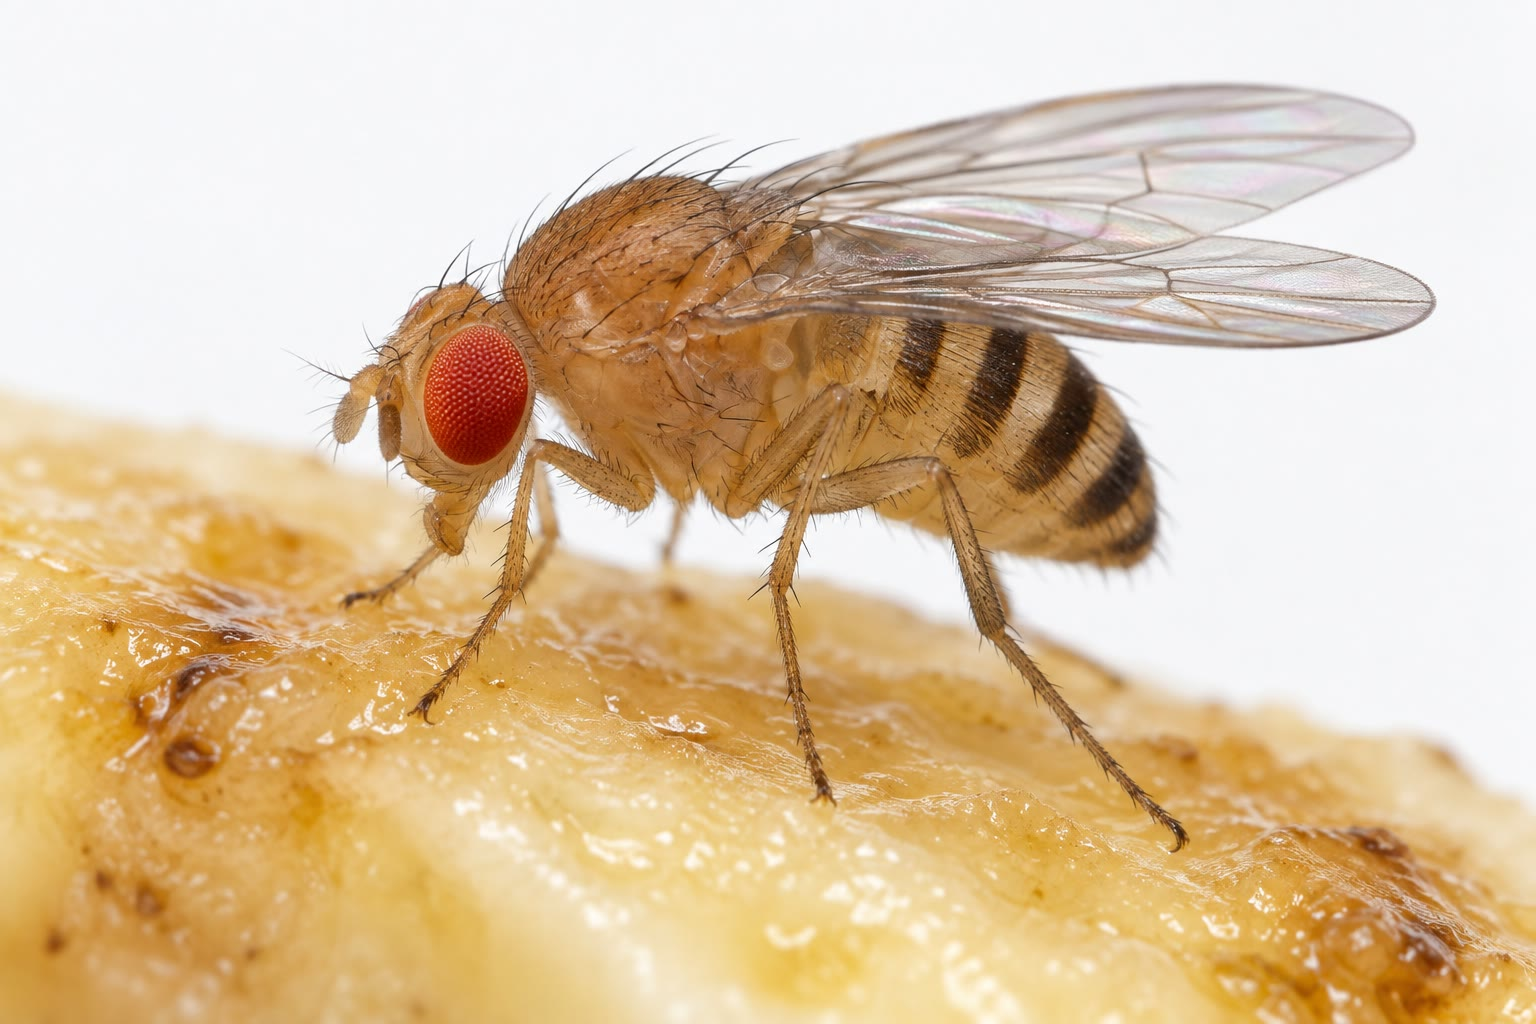
\includegraphics[width=0.5\linewidth]{images/book4/ai/b4-04-drosophila.jpg}

{\small \emph{Drosophila melanogaster}: duas semanas por geração,
centenas de descendentes, quatro pares de cromossomos e um século de
mutantes --- o organismo com o qual se estabeleceram a \omterm{def:b2:meiosis-heredity:linkage}{ligação gênica},
os mapas e a herança ligada ao sexo.}
\end{omfigure}

\section{Cromossomos sexuais e organelas}

\begin{proposition}[A herança ligada ao sexo]\label{prop:b2:meiosis-heredity:sexlinked}
\index{herança ligada ao X}\index{cromossomos sexuais}
Nos mamíferos e nas moscas, a fêmea é $XX$ e o macho $XY$: o $Y$ tem
poucos genes, de modo que um macho tem uma única cópia de cada gene
ligado ao $X$ (é \emph{hemizigoto}) e manifesta o \omterm{def:b2:meiosis-heredity:vocabulary}{alelo} que carrega,
seja \omterm{def:b2:meiosis-heredity:vocabulary}{dominante} ou \omterm{def:b2:meiosis-heredity:vocabulary}{recessivo}. Consequências: os cruzamentos recíprocos
diferem (fêmea de olhos brancos $\times$ macho de olhos vermelhos dá
filhos de olhos brancos e filhas de olhos vermelhos; o cruzamento
inverso dá todos vermelhos); um caráter \omterm{def:b2:meiosis-heredity:vocabulary}{recessivo} ligado ao $X$
(daltonismo vermelho--verde, hemofilia, distrofia muscular de
Duchenne) aparece sobretudo nos homens, é transmitido por mães
portadoras não afetadas e nunca passa de pai para filho (um filho
recebe o $Y$ do pai); um pai transmite seu $X$ a todas as filhas. As
aves, as borboletas e alguns répteis invertem o arranjo (fêmeas $ZW$,
machos $ZZ$); muitos répteis deixam a temperatura decidir; e, nos
mamíferos, um $X$ de cada célula feminina é silenciado ao acaso no
início do desenvolvimento, de modo que uma fêmea heterozigota é um
mosaico (a gata tricolor).
\end{proposition}
\begin{proof}[Evidências]
Morgan (1910) encontrou um único macho de olhos brancos entre milhares
de moscas de olhos vermelhos. Cruzado com fêmeas vermelhas, deu
descendentes todos vermelhos; mas, na geração seguinte, os olhos
brancos reapareceram apenas nos machos, na metade deles. Cruzar um
macho branco com suas filhas vermelhas deu olhos brancos nos dois
sexos. O padrão era exatamente o esperado se o gene estivesse no
cromossomo X, que as fêmeas têm em dose dupla e os machos em dose
simples --- o primeiro gene atribuído a um cromossomo.
\end{proof}

\begin{omfigure}
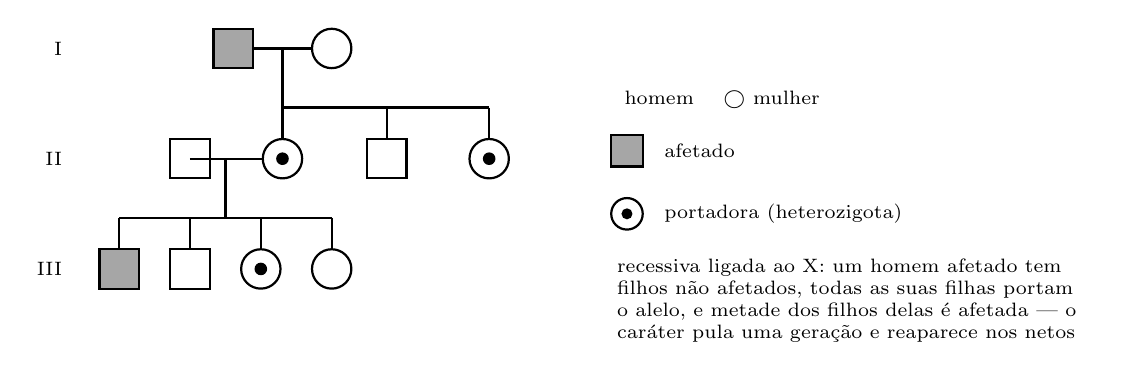
\begin{tikzpicture}[every node/.style={font=\scriptsize}]
  % pedigree: X-linked recessive
  \draw[thick, fill=gray!70] (0,0) rectangle (0.5,0.5); % affected grandfather
  \draw[thick] (1.5,0.25) circle (0.25);
  \draw[thick] (0.5,0.25) -- (1.25,0.25);
  \draw[thick] (0.875,0.25) -- (0.875,-0.5);
  \draw[thick] (0.875,-0.5) -- (3.5,-0.5);
  % children of generation I
  \draw[thick] (0.875,-0.5) -- (0.875,-0.9); \draw[thick, fill=white] (0.875,-1.15) circle (0.25); \fill (0.875,-1.15) circle (0.08);
  \draw[thick] (2.2,-0.5) -- (2.2,-0.9); \draw[thick] (1.95,-1.4) rectangle (2.45,-0.9);
  \draw[thick] (3.5,-0.5) -- (3.5,-0.9); \draw[thick, fill=white] (3.5,-1.15) circle (0.25); \fill (3.5,-1.15) circle (0.08);
  % carrier daughter marries
  \draw[thick] (-0.3,-1.15) -- (0.625,-1.15); \draw[thick] (-0.55,-1.4) rectangle (-0.05,-0.9);
  \draw[thick] (0.15,-1.15) -- (0.15,-1.9); \draw[thick] (-1.2,-1.9) -- (1.5,-1.9);
  \draw[thick] (-1.2,-1.9) -- (-1.2,-2.3); \draw[thick, fill=gray!70] (-1.45,-2.8) rectangle (-0.95,-2.3);
  \draw[thick] (-0.3,-1.9) -- (-0.3,-2.3); \draw[thick] (-0.55,-2.8) rectangle (-0.05,-2.3);
  \draw[thick] (0.6,-1.9) -- (0.6,-2.3); \draw[thick, fill=white] (0.6,-2.55) circle (0.25); \fill (0.6,-2.55) circle (0.08);
  \draw[thick] (1.5,-1.9) -- (1.5,-2.3); \draw[thick, fill=white] (1.5,-2.55) circle (0.25);
  \node[anchor=east] at (-1.8,0.25) {I};
  \node[anchor=east] at (-1.8,-1.15) {II};
  \node[anchor=east] at (-1.8,-2.55) {III};
  % legend
  \node[anchor=west, align=left] at (5,-0.4) {$\square$ homem \quad $\bigcirc$ mulher};
  \draw[thick, fill=gray!70] (5.05,-1.25) rectangle (5.45,-0.85); \node[anchor=west] at (5.6,-1.05) {afetado};
  \draw[thick] (5.25,-1.85) circle (0.2); \fill (5.25,-1.85) circle (0.07); \node[anchor=west] at (5.6,-1.85) {portadora (heterozigota)};
  \node[anchor=north west, align=left, text width=6.2cm] at (5,-2.3) {recessiva ligada ao X: um homem afetado tem filhos não afetados, todas as suas filhas portam o alelo, e metade dos filhos delas é afetada --- o caráter pula uma geração e reaparece nos netos};
\end{tikzpicture}

{\small Heredograma de um caráter \omterm{def:b2:meiosis-heredity:vocabulary}{recessivo} ligado ao X, como a
hemofilia: nenhuma transmissão de pai para filho, filhas portadoras,
netos afetados.}
\end{omfigure}

\begin{method}[Ler um heredograma]\label{met:b2:meiosis-heredity:pedigree}
\index{heredograma}
\begin{enumerate}
  \item Dois genitores não afetados com um filho afetado: o caráter é
        \omterm{def:b2:meiosis-heredity:vocabulary}{recessivo} (os dois genitores são \omterm{def:b2:meiosis-heredity:vocabulary}{heterozigotos}).
  \item Um filho afetado sempre tem um genitor afetado, e o caráter
        aparece em todas as gerações: \omterm{def:b2:meiosis-heredity:vocabulary}{dominante}.
  \item Afetados sobretudo do sexo masculino, transmissão por mães não
        afetadas, nunca de pai para filho: \omterm{def:b2:meiosis-heredity:vocabulary}{recessivo} ligado ao X.
  \item Um pai afetado tem todas as filhas afetadas e nenhum filho
        afetado: \omterm{def:b2:meiosis-heredity:vocabulary}{dominante} ligado ao X.
  \item Transmitido pelas mães a todos os seus filhos, nunca pelos
        pais: mitocondrial.
  \item Em seguida, calcule as probabilidades a partir dos \omterm{def:b2:meiosis-heredity:vocabulary}{genótipos}
        implicados: um casal portadora $\times$ normal tem uma chance de
        $\tfrac14$ de ter um filho afetado a cada nascimento ($\tfrac12$
        menino $\times$ $\tfrac12$ recebe o \omterm{def:b2:meiosis-heredity:vocabulary}{alelo}).
\end{enumerate}
\end{method}

\begin{definition}[Herança extranuclear]\label{def:b2:meiosis-heredity:extranuclear}
\index{herança materna}\index{herança mitocondrial}
As mitocôndrias e os cloroplastos têm seus próprios genomas pequenos,
em muitas cópias por organela e muitas organelas por célula, e vêm
quase inteiramente do óvulo: o espermatozoide contribui com um núcleo
e pouco mais. Seus genes são, portanto, \emph{herdados por via
materna}, sem proporções de segregação: uma mãe transmite o caráter a
todos os seus filhos; um pai, a nenhum. As doenças mitocondriais
humanas (defeitos da cadeia respiratória que afetam os músculos e os
nervos) seguem esse padrão, assim como a variegação de algumas
plantas, em que uma célula-mãe com cloroplastos normais e mutantes os
distribui ao acaso entre as células-filhas, produzindo setores verdes,
brancos e mistos. Como nunca recombinam, as sequências mitocondriais
permitem rastrear as linhagens maternas ao longo do tempo --- a
ferramenta do \cref{ch:b2:phylogenetic-trees}.
\end{definition}

\begin{proposition}[Análise de tétrades]\label{prop:b2:meiosis-heredity:tetrads}
\index{análise de tétrades}\index{tétrade ordenada}
Em alguns fungos (\emph{Neurospora}, \emph{Sordaria}), os quatro
produtos de uma \omterm{def:b2:meiosis-heredity:meiosis}{meiose} permanecem juntos num saco, o \emph{asco}, e em
ordem: uma mitose final dá oito esporos cuja sequência registra as
duas divisões. Para um \omterm{def:b2:meiosis-heredity:vocabulary}{heterozigoto} $A/a$, um asco com o padrão
$4 : 4$ (\emph{segregação na primeira divisão}) não teve crossing-over
entre o gene e seu centrômero --- os \omterm{def:b2:meiosis-heredity:vocabulary}{alelos} se separaram na anáfase I;
um padrão $2 : 2 : 2 : 2$ ou $2 : 4 : 2$ (\emph{segregação na segunda
divisão}) teve um, de modo que os \omterm{def:b2:meiosis-heredity:vocabulary}{alelos} só se separaram na anáfase
II. A distância do gene ao centrômero é metade da porcentagem de ascos
de segunda divisão, pois um crossing-over recombina apenas duas das
quatro cromátides. As tétrades mostram também diretamente que a
recombinação é recíproca: toda cromátide recombinante tem sua parceira
complementar no mesmo asco.
\end{proposition}

\begin{omfigure}
\begin{tikzpicture}[every node/.style={font=\scriptsize}]
  \foreach \dx/\pat/\lab in {0/{omDef,omDef,omDef,omDef,omThm,omThm,omThm,omThm}/{$4:4$, sem crossing-over:\\segregação na\\1.\textsuperscript{a} divisão}, 4.5/{omDef,omDef,omThm,omThm,omDef,omDef,omThm,omThm}/{$2:2:2:2$, crossing-over entre\\o gene e o centrômero}, 9/{omDef,omDef,omThm,omThm,omThm,omThm,omDef,omDef}/{$2:4:2$, crossing-over:\\segregação na 2.\textsuperscript{a} divisão}} {
    \begin{scope}[xshift=\dx cm]
      \draw[thick, rounded corners=6pt] (0,0) rectangle (0.8,4.2);
      \foreach \c [count=\i] in \pat { \fill[\c] (0.4,4.2-0.5*\i+0.02) circle (0.2); }
      \node[below, align=center] at (0.4,-0.1) {\lab};
    \end{scope}
  }
  \node[anchor=west, align=left, text width=2.6cm] at (12.4,3.2) {ascos ordenados de \emph{Sordaria}; esporos azuis e vermelhos levam os dois alelos};
\end{tikzpicture}

{\small \omterm{prop:b2:meiosis-heredity:tetrads}{Tétrades ordenadas}. Sem crossing-over entre o gene e seu
centrômero, os \omterm{def:b2:meiosis-heredity:vocabulary}{alelos} se separam na primeira divisão e os oito esporos
dão $4 : 4$; com um, separam-se na segunda divisão e o asco dá
$2 : 2 : 2 : 2$ ou $2 : 4 : 2$.}
\end{omfigure}

\section{Exercícios}

\begin{exercise}[$\star$]\label{exo:b2:meiosis-heredity:1}
Liste quatro diferenças entre a mitose e a \omterm{def:b2:meiosis-heredity:meiosis}{meiose} (número de divisões,
pareamento, produtos, identidade genética dos produtos).
\end{exercise}

\begin{exercise}[$\star$]\label{exo:b2:meiosis-heredity:2}
Quantos gametas cromossomicamente distintos uma pessoa pode produzir
apenas por \omterm{thm:b2:meiosis-heredity:mixing}{segregação independente}? E uma drosófila ($n = 4$)? E uma
ervilha ($n =
7$)?
\end{exercise}

\begin{exercise}[$\star$]\label{exo:b2:meiosis-heredity:3}
Nas ervilhas, alto ($T$) é \omterm{def:b2:meiosis-heredity:vocabulary}{dominante} sobre anão. Dê as proporções
fenotípicas e genotípicas de $Tt \times Tt$ e de $Tt \times tt$. Como
descobrir se uma planta alta é $TT$ ou $Tt$?
\end{exercise}

\begin{exercise}[$\star$]\label{exo:b2:meiosis-heredity:4}
Defina \omterm{def:b2:meiosis-heredity:linkage}{ligação gênica}, \omterm{def:b2:meiosis-heredity:linkage}{frequência de recombinação} e \omterm{def:b2:meiosis-heredity:linkage}{centimorgan}. Por
que dois genes situados no mesmo cromossomo podem, ainda assim,
segregar como se fossem independentes?
\end{exercise}

\begin{exercise}[$\star\star$]\label{exo:b2:meiosis-heredity:5}
O \omterm{thm:b2:meiosis-heredity:mendel}{cruzamento di-híbrido} de Mendel deu $315$ lisas amarelas, $108$
lisas verdes, $101$ rugosas amarelas e $32$ rugosas verdes. Teste a
hipótese $9 : 3 : 3 :
1$ com o $\chi^2$ (3 graus de liberdade, valor crítico
$7.81$).
\end{exercise}

\begin{exercise}[$\star\star$]\label{exo:b2:meiosis-heredity:6}
Um di-híbrido $AB/ab$ submetido a cruzamento-teste dá $412$ $AB$,
$388$ $ab$, $103$
$Ab$, $97$ $aB$. Os genes estão ligados? Calcule a \omterm{def:b2:meiosis-heredity:linkage}{frequência de
recombinação} e a distância de mapa; o que daria o di-híbrido $Ab/aB$?
\end{exercise}

\begin{exercise}[$\star\star$]\label{exo:b2:meiosis-heredity:7}
Usando a função de Haldane, converta $r = 0.20$ e $r = 0.45$ em
distâncias de mapa, e \qty{30}{cM} e \qty{100}{cM} em frações de
recombinação. Comente quais conversões importam na prática.
\end{exercise}

\begin{exercise}[$\star\star$]\label{exo:b2:meiosis-heredity:8}
Em \emph{Drosophila}, olho branco ($w$) é \omterm{def:b2:meiosis-heredity:vocabulary}{recessivo} ligado ao X. Dê os
descendentes, por sexo e \omterm{def:b2:meiosis-heredity:vocabulary}{fenótipo}, de (a) fêmea branca $\times$ macho
vermelho, (b) fêmea vermelha heterozigota $\times$ macho branco, (c) o
cruzamento das filhas de (a) com seus irmãos.
\end{exercise}

\begin{exercise}[$\star\star$]\label{exo:b2:meiosis-heredity:9}
Duas linhagens puras de ervilha-de-cheiro de flores brancas, cruzadas,
dão descendentes todos púrpuras, que, autofecundados, dão $9$
púrpuras : $7$ brancas. Explique com dois genes, dê os \omterm{def:b2:meiosis-heredity:vocabulary}{genótipos} das duas
linhagens parentais e preveja o resultado do cruzamento-teste do
híbrido púrpura.
\end{exercise}

\begin{exercise}[$\star\star\star$]\label{exo:b2:meiosis-heredity:10}
Um cruzamento-teste de três pontos dá: $+++$ 480, $abc$ 470, $+bc$ 11,
$a++$ 9, $++c$ 118, $ab+$ 112, $+b+$ 1, $a+c$ 1 (total 1202).
Encontre a ordem dos genes, as duas distâncias, o coeficiente de
coincidência e a interferência.
\end{exercise}

\begin{exercise}[$\star\star\star$]\label{exo:b2:meiosis-heredity:11}
Em \emph{Sordaria}, um cruzamento de uma linhagem de esporos pretos
com uma de esporos castanho-claros dá $700$ ascos de padrão $4 : 4$ e
$300$ de padrões $2 : 2 : 2 : 2$ ou $2 : 4 : 2$. Calcule a distância
do gene da cor dos esporos ao seu centrômero e explique por que é
necessário o fator um meio. Desenhe as cromátides de uma \omterm{def:b2:meiosis-heredity:meiosis}{meiose} que dê
$2 : 4 : 2$.
\end{exercise}

\begin{exercise}[$\star\star\star$]\label{exo:b2:meiosis-heredity:12}
O avô materno de uma mulher tinha hemofilia; ninguém mais na família é
afetado. Qual é a probabilidade de ela ser portadora? Sabendo que ela
teve dois filhos saudáveis, qual é essa probabilidade agora? Mostre o
raciocínio.
\end{exercise}

\section{Problema: Cruzamentos na sala das moscas}

\begin{problem}[{Problema de fim de semana --- cruzamentos de
\emph{Drosophila} analisados da proporção mono-híbrida a um mapa de
três pontos, e um heredograma humano calculado, até o mapa de três
genes ligados ao X e sua interferência}]
\label{pb:b2:meiosis-heredity:1}
Asa vestigial ($vg$) e corpo ébano ($e$) são \omterm{def:b2:meiosis-heredity:vocabulary}{recessivos} e estão em
autossomos diferentes; corpo preto ($b$) e $vg$ são \omterm{def:b2:meiosis-heredity:vocabulary}{recessivos} e estão
ambos no cromossomo 2; corpo amarelo ($y$), olho branco ($w$) e asa
miniatura ($m$) são \omterm{def:b2:meiosis-heredity:vocabulary}{recessivos} e ligados ao X. Valores críticos de
$\chi^2$ a \qty{5}{\%}: $3.84$ (1 g.l.), $7.81$ (3 g.l.).

\medskip
\noindent\textbf{Parte I --- Dois genes autossômicos.}
Uma mosca vestigial pura é cruzada com uma mosca ébano pura; as $F_1$
são todas de tipo selvagem; $1600$ moscas $F_2$ são classificadas:
$892$ selvagens, $309$ vestigiais, $296$ ébano, $103$ vestigiais
ébano.
\begin{enumerate}
  \item Dê os \omterm{def:b2:meiosis-heredity:vocabulary}{genótipos} dos genitores, da $F_1$ e dos gametas
        da $F_1$.
  \item Calcule as contagens esperadas sob \omterm{thm:b2:meiosis-heredity:mixing}{segregação independente}.
  \item Calcule o $\chi^2$ e conclua.
  \item Que fração das moscas $F_2$ de tipo selvagem é homozigota nos
        dois locos?
  \item A $F_1$ é submetida a cruzamento-teste com uma mosca vestigial
        ébano: preveja as quatro classes e suas proporções.
  \item Moscas ébano criadas a \qty{29}{\celsius} são mais claras que a
        \qty{18}{\celsius}. O que isso diz sobre a relação entre
        \omterm{def:b2:meiosis-heredity:vocabulary}{genótipo} e \omterm{def:b2:meiosis-heredity:vocabulary}{fenótipo}?
\end{enumerate}

\medskip
\noindent\textbf{Parte II --- Dois genes ligados.}
Uma mosca preta pura é cruzada com uma mosca vestigial pura; as fêmeas
$F_1$ são submetidas a cruzamento-teste com machos pretos vestigiais:
$965$ pretas, $944$ vestigiais, $206$ pretas vestigiais, $185$ de tipo
selvagem.
\begin{enumerate}[resume]
  \item Escreva o \omterm{def:b2:meiosis-heredity:vocabulary}{genótipo} da $F_1$, mostrando quais \omterm{def:b2:meiosis-heredity:vocabulary}{alelos} estão no
        mesmo cromossomo.
  \item Identifique as classes parentais e recombinantes e explique
        por que o tipo selvagem é aqui um \emph{recombinante}.
  \item Calcule $r$ e a distância de mapa.
  \item Corrija-a com a função de Haldane.
  \item O mesmo cruzamento, com os \emph{machos} $F_1$ submetidos a
        cruzamento-teste, dá apenas duas classes, pretos e vestigiais,
        em números iguais. O que isso mostra sobre a \omterm{def:b2:meiosis-heredity:meiosis}{meiose} dos machos
        de mosca?
  \item Preveja as classes e as proporções se a fêmea $F_1$ viesse de
        um cruzamento preto vestigial $\times$ selvagem.
\end{enumerate}

\medskip
\noindent\textbf{Parte III --- Um heredograma humano.}
A hemofilia A é recessiva ligada ao X. Um homem com hemofilia tem uma
filha, que se casa com um homem não afetado.
\begin{enumerate}[resume]
  \item Qual é o \omterm{def:b2:meiosis-heredity:vocabulary}{genótipo} da filha, e por que ele é certo?
  \item Probabilidade de que seu primeiro filho seja um menino afetado.
  \item Probabilidade de que uma filha dela seja portadora.
  \item Probabilidade de que, entre seus três filhos, nenhum seja
        afetado.
  \item Explique por que a doença nunca passa de pai para filho, e
        como uma mulher poderia ser afetada.
  \item A irmã do homem afetado tem dois filhos saudáveis; a mãe deles
        (a mãe do homem) era portadora. Calcule a probabilidade de que a
        irmã seja portadora, antes e depois de levar em conta seus
        filhos.
\end{enumerate}

\medskip
\noindent\textbf{Parte IV --- Três genes ligados ao X.}
Uma fêmea $y\,w\,m/+\,+\,+$ é cruzada com um macho $y\,w\,m$; seus
$2000$ filhos são classificados: $+++$ 853, $ywm$ 833, $y++$ 24,
$+wm$ 26, $yw+$ 128, $++m$ 132, $+w+$ 2, $y+m$ 2.
\begin{enumerate}[resume]
  \item Por que os filhos podem ser classificados diretamente, sem
        cruzamento-teste?
  \item Identifique as classes parentais e as de crossing-over duplo e
        deduza a ordem dos genes.
  \item Calcule as duas \omterm{def:b2:meiosis-heredity:linkage}{frequências de recombinação} e desenhe o mapa.
  \item Calcule o número esperado de crossing-overs duplos, o
        coeficiente de coincidência e a interferência.
  \item Calcule a \omterm{def:b2:meiosis-heredity:linkage}{frequência de recombinação} entre os dois genes
        externos diretamente a partir dos dados, e explique por que ela
        é menor que a soma das duas distâncias.
  \item Como seriam as filhas desse cruzamento, e por que são inúteis
        para o mapeamento?
  \item Enuncie o resultado: o mapa dos três genes e a interferência.
\end{enumerate}
\end{problem}
